%% PeerJ manuscript skeleton based on the official Overleaf template.
%% Note: wlpeerj.cls should be present in this directory (download from template source).
\documentclass[fleqn,10pt,lineno]{wlpeerj}

\title{Complex Layers of Sparse Formal Neurons for High-Dimensional Classification}

\author[1]{Jerzy Krawczuk}
\author[2]{Leon Bobrowski}
\affil[1]{Faculty of Computer Science, Bialystok University of Technology, Wiejska 45A, Bialystok, Poland}
\affil[2]{Institute of Biocybernetics and Biomedical Engineering, PAS, Warsaw, Poland}
\corrauthor[1]{Jerzy Krawczuk}{j.krawczuk@pb.edu.pl}

% Keywords can be provided in the submission system metadata.

\begin{abstract}
\textbf{Background.}
High-dimensional gene-expression datasets remain difficult classification benchmarks because they combine
very small sample sizes with thousands of correlated features. Sparse linear models are attractive in this
setting because they can preserve interpretability, but their predictive behavior may depend strongly on
the way sparsity is imposed and on how successive feature subsets are constructed. This study examines the
behavior of successive sparse neurons in a complex-layer construction, with emphasis on how signal, sparsity,
and noise evolve across neuron depth.

\textbf{Methods.}
We study two complementary benchmarks. The first is the classical colon cancer microarray dataset
containing 62 samples, 2,000 features, and two diagnostic classes. The second is a synthetic binary dataset
with known informative features, redundant correlated features, and noise features, together with an explicit
ranking of informative-feature strengths. Three linear learners are evaluated within the same complex-layer
protocol: \texttt{cpl} (convex piecewise-linear; hinge loss with L1 regularization), \texttt{svm}
(squared hinge loss with L1 regularization), and \texttt{logreg} (logistic loss with L1 regularization).
In each layer, one sparse neuron is trained and the
features selected by that neuron are removed before fitting the next one. Performance is assessed using
repeated stratified cross-validation. For each neuron depth, we report predictive accuracy, sparsity,
weighted voting, and---for the synthetic benchmark---feature-recovery analysis.

\textbf{Results.}
On \texttt{colon\_cancer}, low-feature first-neuron solutions often benefited from later neurons:
\texttt{cpl} improved from 0.8438 at $n=1$ to 0.8498 at $n=4$, \texttt{svm} from 0.8195 to 0.8512 at $n=3$,
and \texttt{logreg} from 0.8545 to 0.8657 at $n=4$. In high-feature regimes, the first neuron more often captured
most of the predictive signal immediately, although high-feature \texttt{cpl} still improved from 0.8726 at $n=1$
to 0.8921 at $n=3$. A train-fold balanced-accuracy weighted vote gave similar conclusions and slightly
improved low-feature \texttt{svm} on the colon cancer benchmark (0.8545 at $n=4$). On the synthetic benchmark, low-feature
configurations of \texttt{cpl}, \texttt{svm}, and \texttt{logreg} reached their best unweighted accuracies at
$n=12$, $n=11$, and $n=5$, respectively. Ground-truth-aware metrics showed two distinct modes: broad first
neurons recovered more informative signal at once, whereas narrower first neurons recovered informative
structure more gradually across successive neurons.

\textbf{Conclusions.}
This study provides a reproducible benchmarking protocol for layered sparse linear classifiers
that combines a realistic microarray benchmark with a diagnostic synthetic benchmark of known signal structure.
Its main value is methodological: it treats neuron depth as an analyzable model dimension rather than assuming
that deeper voting must improve monotonically. The results indicate that useful signal is usually concentrated
in the first few neurons, but the way it is distributed across depth depends strongly on the learner and on
the feature-count regime.
\end{abstract}

\begin{document}
\flushbottom
\maketitle
\thispagestyle{empty}

\section*{Introduction}

High-dimensional biological datasets are challenging for linear classifiers due to the small-sample, many-feature
regime and strong feature redundancy. Layered sparse classifiers provide an interpretable approach by learning
sequential neurons and removing selected features after each step.
This setting is also a classical use case for sparse linear modeling and embedded feature selection
\cite{tibshirani1996lasso,ng2004l1l2,saeys2007review}.

This work focuses on two complementary benchmarks. The first is the \texttt{colon\_cancer} microarray dataset,
one of the canonical benchmarks in bioinformatics and machine learning for high-dimensional classification
\cite{alon1999,guyon2002,dudoit2002,li2004}. It originates from the colon tumor vs.\ normal tissue profiling
study published in 1999 \cite{alon1999}. Across more than two decades, this benchmark has been repeatedly used
to evaluate feature selection, sparse linear models, and stability of classification under strong
$p \gg n$ conditions \cite{guyon2002,dudoit2002,li2004}. In comparative studies, \texttt{colon\_cancer}
typically yields high-80\% to mid-90\% accuracy ranges depending on validation protocol and feature-selection
strategy \cite{guyon2002,dudoit2002,li2004}.

The second benchmark is synthetic and is introduced for a different purpose. Real biological datasets provide
realistic distributional complexity, but they do not reveal the true predictive contribution of each feature.
As a consequence, they are suitable for measuring predictive performance and sparsity, but not for directly
measuring whether a method recovers the genuinely informative variables before drifting toward redundant or
purely noisy ones. This distinction is particularly important in high-dimensional gene-expression studies,
where feature selection and classifier evaluation can become confounded by selection bias if the protocol is
not carefully separated across training and test data \cite{ambroise2002,krawczuk2016feature}. To address
this limitation, we add a synthetic binary benchmark with known informative
features, controlled redundant features, and a predefined ranking of informative-feature strengths.
This perspective is also aligned with recent work emphasizing that feature-selection stability should be
treated as an important evaluation dimension in high-dimensional classification, not merely as a secondary
diagnostic after predictive accuracy \cite{lukaszuk2024importance}.

We compare three methods under the same protocol:
\texttt{cpl}, \texttt{svm}, and \texttt{logreg}. The goal is to assess how predictive performance, sparsity,
computational cost, and feature-recovery behaviour evolve across successive neurons in a controlled repeated
cross-validation setup.
The compared learners are all grounded in well-established sparse linear classification frameworks, including
L1-regularized logistic models and large-scale linear classifiers \cite{friedman2010glmnet,fan2008liblinear}.

Rather than assuming that aggregating many neurons must monotonically improve classification, we study a more
basic and more informative question: what does each next neuron contribute? In particular, we ask how much
predictive signal is captured by the first neurons, when later neurons still add complementary information, and
when they become dominated by redundant or noisy features.

Main contributions:
\begin{enumerate}[noitemsep]
\item A unified complex-layer framework evaluated with three linear sparse learners.
\item A repeated cross-validation benchmark on the classical \texttt{colon\_cancer} microarray dataset.
\item A synthetic benchmark with known feature relevance and known ranking of signal strengths.
\item Reproducible reporting of neuron-by-neuron accuracy, sparsity, weighted voting, and feature-recovery
diagnostics.
\end{enumerate}

\section*{Methods}

\subsection*{Dataset}
We use two datasets: one real benchmark and one synthetic benchmark.

\subsubsection*{Real-data benchmark: colon cancer}
We use the colon cancer dataset, originally introduced by \cite{alon1999}. It is a gene-expression
microarray benchmark built from colon tumor and normal tissue samples.
In the commonly used machine-learning representation, the data matrix contains:
\begin{itemize}[noitemsep]
\item 62 objects (samples),
\item 2,000 gene-expression features,
\item binary labels: \texttt{tumor} (40) and \texttt{normal} (22).
\end{itemize}

The dataset originates from the Alon et al. colon adenocarcinoma study published in 1999 \cite{alon1999}
and has since become a long-standing reference problem for sparse learning and feature selection in
bioinformatics, with representative comparative results in \cite{guyon2002,dudoit2002,li2004}.

\subsubsection*{Synthetic benchmark with known signal strength}
To assess feature recovery directly, we additionally generate a synthetic binary classification dataset with
a known ground-truth definition. The synthetic benchmark is designed to separate predictive performance
from feature-discovery quality.

The guiding idea is simple. The benchmark should contain a small set of truly informative variables, a larger
set of variables that are correlated with the true signal but are not themselves primary signal variables, and
many unrelated noise variables. This lets us ask whether later neurons recover new informative signal or only
move toward redundant and noisy features.

The final synthetic dataset used in this study has:
\begin{itemize}[noitemsep]
\item 100 samples,
\item 2,000 features in total,
\item balanced classes: 50 negative and 50 positive samples,
\item 12 informative features,
\item 36 redundant features,
\item 1,952 noise features.
\end{itemize}

The construction is based on three latent signal sources. For each sample $i$ and source
$b \in \{1,2,3\}$, a latent value $z_{ib}$ is drawn from a standard normal distribution. The three sources have
decreasing strengths
\[
s=(1.2,\;0.9,\;0.6),
\]
so source 1 is strongest and source 3 is weakest. The class score is generated directly from these latent
signals:
\[
r_i=\sum_{b=1}^{3}s_b z_{ib}+\eta_i,
\]
where $\eta_i$ is Gaussian label noise with scale 0.55. The score is thresholded at its median, yielding
exactly 50 negative and 50 positive samples.

Each latent source is then represented in the observed feature matrix by four truly informative features and
twelve correlated redundant features. Thus, the observed signal-related part of the feature matrix has
$3\times4=12$ informative features and $3\times12=36$ redundant features; the remaining 1,952 features are
independent noise. Informative features are indexed first, followed by redundant features, and finally by noise
features.

For an informative feature $j$ assigned to source $b$, the observed value is a noisy measurement of the
corresponding latent source:
\[
x_{ij}=w_j z_{ib}+\epsilon_{ij}.
\]
The feature noise is Gaussian with scale 0.2. The informative weights decrease in absolute value within each
signal source and alternate in sign. Thus, informative features have a known order of importance both across
signal sources and within each source, while the benchmark does not reduce to selecting only positively
correlated variables. The exact informative-feature weights and feature-index mapping are fixed by the
benchmark definition.

Redundant features are also assigned to one signal source. Each redundant feature is generated as a correlated
surrogate of one informative feature from that source and also receives a smaller contribution from the same
latent value $z_{ib}$. The redundant-feature noise scale is 0.3. These variables can be
predictive because they are correlated with the signal, but they are not counted as truly informative in the
ground truth.

Class labels are therefore generated from the three latent signal sources, not from all 2,000 observed features. This
preserves a known latent signal structure while allowing the observed feature matrix to contain informative,
redundant, and purely noisy variables.

After generation, all feature columns are standardized by z-scoring. As a result, feature variances are on a
common scale, but the effective signal-to-noise ratios remain different across informative, redundant, and
noise features.

The benchmark definition specifies the exact indices of informative, redundant, and noise features. This makes it
possible to evaluate not only predictive accuracy, but also how many of the 12 ground-truth informative
features are recovered by each neuron and by the cumulative sequence of neurons.

\subsection*{Model family}
The core model is a complex-layer classifier that sequentially trains sparse linear neurons and removes selected
features after each neuron. This construction follows the Complex Layers of Formal Neurons line of work
\cite{bobrowski2021,bobrowski2022}. For analysis, we treat neuron depth $n$ as a model dimension in its own
right. For each depth, we inspect both the prediction of the $n$-th neuron itself and the cumulative prediction
obtained by majority voting over the first $n$ neurons.

The label \texttt{cpl} refers to the convex piecewise-linear base learner used in this study. Its
objective combines hinge loss with L1 regularization; both terms are convex piecewise-linear, so the resulting
sparse linear neuron can be trained as a linear programming problem. It is evaluated inside the same
complex-layer protocol as two standard sparse linear baselines:
\begin{itemize}[noitemsep]
\item \texttt{cpl}: convex piecewise-linear neuron trained with an LP-based hinge + L1 formulation.
\item \texttt{svm}: LinearSVC (squared hinge loss + L1 regularization).
\item \texttt{logreg}: logistic regression with L1 regularization.
\end{itemize}
The use of L1-type regularization is motivated by its long-standing role in sparse estimation and feature
selection for high-dimensional problems \cite{tibshirani1996lasso,ng2004l1l2}. For logistic regression, the
computational perspective is closely related to regularization-path methods such as \texttt{glmnet}
\cite{friedman2010glmnet}, while the practical large-scale linear classification setting is represented by
\texttt{LIBLINEAR} \cite{fan2008liblinear}.

\subsection*{Evaluation protocol}
For both benchmarks, we use repeated stratified cross-validation with a fixed random seed.
Both benchmarks reported in this manuscript use 10 folds and 10 repeats, giving 100 train/test splits for
each dataset and model configuration.
The split-wise protocol is important in this setting because feature selection bias is a well-known failure
mode in high-dimensional gene-expression studies when selection and evaluation are not strictly separated
\cite{ambroise2002,krawczuk2016feature}.

\subsection*{Computational environment}
All experiments were implemented in Python and are distributed with the manuscript repository. The submitted
artifact specifies Python 3.13 or 3.14 with Poetry-managed dependencies; the final local verification used
Python 3.14.3 and Poetry 2.3.2. Package versions are pinned in \texttt{poetry.lock}, including
\texttt{numpy}, \texttt{scipy}, \texttt{scikit-learn}, \texttt{pandas}, and \texttt{matplotlib}. The paper-scale
runs were executed on a MacBook Air (Apple M2, 2022; 16 GB RAM) running macOS Tahoe 26.5.1, and each run
records wall-clock time and peak resident memory in its \texttt{run\_stats.json} metadata. The repository
scripts are the authoritative workflow for regenerating raw predictions, metric tables, and figures from the
input datasets.

\subsection*{Regularization calibration}
Because the three base learners use different optimization schemes and induce sparsity at different rates,
their regularization parameters are not directly comparable on a shared numerical scale. To make the comparison
more interpretable, we calibrate two representative regularization settings for each model on each dataset.

The calibration procedure is intentionally simple. For a given dataset, model, and value of $C$, we fit only
the first neuron and record the number of selected features. We then choose two values of $C$:
\begin{itemize}[noitemsep]
\item a \textbf{low-feature} setting targeting approximately five selected features in the first neuron;
\item a \textbf{high-feature} setting targeting approximately twenty-five selected features in the first neuron.
\end{itemize}

This calibration does not make the models equivalent, and it is not intended to support a strict ranking of
the base learners. Its purpose is to place each learner in two interpretable feature-count regimes and then
study how that learner behaves as successive neurons are added. Realized first-neuron widths can still differ
across learners under cross-validation, especially when the sparsity path changes abruptly with $C$.
This choice follows the broader methodological view that comparisons between sparse learners should distinguish
the induced first-neuron width from the raw numerical value of the regularization parameter itself
\cite{ng2004l1l2,saeys2007review}.

\begin{table}[ht]
\centering
\begin{tabular}{llrrrr}
\toprule
Dataset & Model & $C_{\mathrm{low}}$ & Features & $C_{\mathrm{high}}$ & Features \\
\midrule
Colon cancer & \texttt{cpl} & 0.03 & 6 & 0.08 & 24 \\
Colon cancer & \texttt{svm} & 1.2 & 5 & 6.0 & 25 \\
Colon cancer & \texttt{logreg} & 3.5 & 6 & 6.4 & 26 \\
Synthetic benchmark & \texttt{cpl} & 0.035 & 4 & 0.05 & 27 \\
Synthetic benchmark & \texttt{svm} & 2.0 & 6 & 3.5 & 26 \\
Synthetic benchmark & \texttt{logreg} & 5.0 & 7 & 9.2 & 25 \\
\bottomrule
\end{tabular}
\caption{Calibration of regularization strength by first-neuron feature count. For each dataset and model, the
parameter $C_{\mathrm{low}}$ was selected to produce roughly five selected features in the first neuron, and
$C_{\mathrm{high}}$ to produce roughly twenty-five selected features. The reported feature counts come from a
single fit of the first neuron on the full dataset and are used only to define comparable low-feature and
high-feature regimes before repeated cross-validation.}
\label{tab:regularization_calibration}
\end{table}

For each split:
\begin{enumerate}[noitemsep]
\item The model is trained only on the training fold.
\item A sequence of up to 31 neurons is fitted.
\item After each neuron fit, features with non-zero coefficients are removed from the candidate pool
for subsequent neurons.
\item Predictions are computed on the held-out test fold.
\end{enumerate}

For each split and neuron depth $n$:
\begin{itemize}[noitemsep]
\item \textbf{vote prediction}: majority vote over the first $n$ neurons;
\item \textbf{weighted vote prediction}: vote over the first $n$ neurons with weights estimated only from the
training fold;
\item \textbf{neuron prediction}: prediction of the $n$-th neuron only.
\end{itemize}

For the weighted vote, each neuron receives a non-negative quality score derived from its training-fold
balanced accuracy:
\[
q_j=\max\left(0,\mathrm{BA}^{\mathrm{train}}_j-0.5\right),
\qquad
w_j=\frac{q_j}{\sum_{\ell=1}^{n} q_\ell}.
\]
If all $q_j$ are zero, uniform weights are used. The chance-level offset of 0.5 makes neurons with no
above-chance balanced accuracy contribute zero weight. Because all weights are computed on the training fold,
this procedure does not use held-out labels.

Then, for each neuron index $n$, metrics are averaged over all 100 splits.

For each neuron depth, we report the mean accuracy of the majority vote, the mean held-out accuracy of the
training-quality weighted vote, the accuracy of the $n$-th neuron alone, and the mean number of features
selected by that neuron.

For the synthetic benchmark, the known set of 12 informative features also allows feature-recovery analysis.
Feature precision measures what fraction of the selected features are truly informative, while feature recall
measures what fraction of the 12 informative features have been recovered. We use both per-neuron and
cumulative recall to assess whether later neurons add new signal or mainly move toward redundant and noisy
variables.
This emphasis goes beyond pure prediction accuracy and is consistent with prior arguments that feature
selection quality and stability deserve explicit evaluation in high-dimensional settings
\cite{saeys2007review,nogueira2018stability,lukaszuk2024importance}.

For binary labels $y_i \in \{-1,+1\}$ and linear score $f(x_i)=w^\top x_i + b$, the objective forms are:
\[
\texttt{cpl}: \quad
\min_{w,b}\ \frac{1}{N}\sum_{i=1}^{N}\max\!\left(0,\,1-y_i f(x_i)\right) + \lambda\lVert w\rVert_1
\]
\[
\texttt{svm}: \quad
\min_{w,b}\ \frac{1}{N}\sum_{i=1}^{N}\max\!\left(0,\,1-y_i f(x_i)\right)^2 + \lambda\lVert w\rVert_1
\]
\[
\texttt{logreg}: \quad
\min_{w,b}\ \frac{1}{N}\sum_{i=1}^{N}\log\!\left(1+\exp(-y_i f(x_i))\right) + \lambda\lVert w\rVert_1
\]

All metrics are reported as mean and standard deviation across splits.

The nominal maximum number of neurons is set to 31; training may stop earlier if no additional non-zero
feature set can be produced.

\section*{Results}

The tables below summarize within-learner trajectories rather than a strict leaderboard between base learners,
because the calibrated first-neuron widths are similar but not identical across models.

\begin{table}[ht]
\centering
\small
\setlength{\tabcolsep}{3.5pt}
\begin{tabular}{llrr@{\hspace{1.8em}}rr@{\hspace{1.8em}}r}
\toprule
Model & Regime & \multicolumn{2}{c@{\hspace{1.8em}}}{$n=1$} & \multicolumn{2}{c@{\hspace{1.8em}}}{Best $n$} & Built \\
\cmidrule(lr){3-4}\cmidrule(lr){5-6}
 & & Features & Accuracy & $n$ & Accuracy & neurons \\
\midrule
\texttt{cpl} & $C_{\mathrm{low}}$ & 4.43 & 0.7690 & 4 & 0.7710 & 13 \\
\texttt{svm} & $C_{\mathrm{low}}$ & 5.73 & 0.8538 & 3 & 0.8545 & 30 \\
\texttt{logreg} & $C_{\mathrm{low}}$ & 3.82 & 0.8524 & 1 & 0.8524 & 3 \\
\midrule
\texttt{cpl} & $C_{\mathrm{high}}$ & 23.42 & 0.8245 & 4 & 0.8493 & 31 \\
\texttt{svm} & $C_{\mathrm{high}}$ & 21.54 & 0.8326 & 3 & 0.8514 & 31 \\
\texttt{logreg} & $C_{\mathrm{high}}$ & 23.89 & 0.8667 & 1 & 0.8667 & 8 \\
\bottomrule
\end{tabular}
\caption{Summary of the repeated-CV results on the colon cancer benchmark. The table reports the average width and
mean vote accuracy of the first neuron, the neuron depth at which the best mean vote accuracy was achieved,
the corresponding mean accuracy, and the realized number of neurons.}
\label{tab:colon_summary}
\end{table}

\subsection*{Colon cancer benchmark}
On the colon cancer benchmark, the low-feature regime showed learner-specific behavior across the first few
successive neurons.
For \texttt{cpl} with $C_{\mathrm{low}}$, the mean vote accuracy increased from 0.7690 for the first neuron to
0.7710 at $n=4$, while the average first-neuron width was 4.43 features.
For \texttt{svm} with $C_{\mathrm{low}}$, accuracy increased slightly from 0.8538 at $n=1$ to 0.8545 at $n=3$.
For \texttt{logreg} with $C_{\mathrm{low}}$, the best mean vote accuracy was already obtained by the first neuron
(0.8524), and only three neurons were built before the feature space was exhausted under this setting.

The high-feature regime produced a different pattern.
For \texttt{cpl} with $C_{\mathrm{high}}$, the mean vote accuracy improved from 0.8245 at $n=1$ to 0.8493 at
$n=4$.
For \texttt{svm} with $C_{\mathrm{high}}$, accuracy increased from 0.8326 at $n=1$ to 0.8514 at $n=3$.
In contrast, \texttt{logreg} with $C_{\mathrm{high}}$ achieved the highest colon cancer accuracy in this
evaluation at the first neuron (0.8667), and additional neurons did not improve the vote.

The weighted vote based on training-fold balanced accuracy did not materially change the qualitative pattern of
the colon cancer results. It matched the best unweighted result for low-feature \texttt{svm}
(0.8545 at $n=3$), low-feature \texttt{logreg} (0.8524 at $n=1$), high-feature \texttt{svm} (0.8514 at $n=3$),
and high-feature \texttt{logreg} (0.8667 at $n=1$).
For \texttt{cpl}, the weighted vote was very close to the unweighted vote, reaching 0.7698 at $n=4$ in the
low-feature regime and 0.8481 at $n=4$ in the high-feature regime.

Taken together, the colon cancer results indicate that useful complementary signal often appears in
the first few neurons, but the benefit of depth depends strongly on the base learner and feature-count regime.
The trajectory figures therefore focus on the low-feature regime, where neuron depth is most informative and
successive neurons have the clearest opportunity to add complementary signal. High-feature regimes are summarized
in Table~\ref{tab:colon_summary} and discussed in the text as a contrasting case.

\begin{figure}[!htbp]
\centering
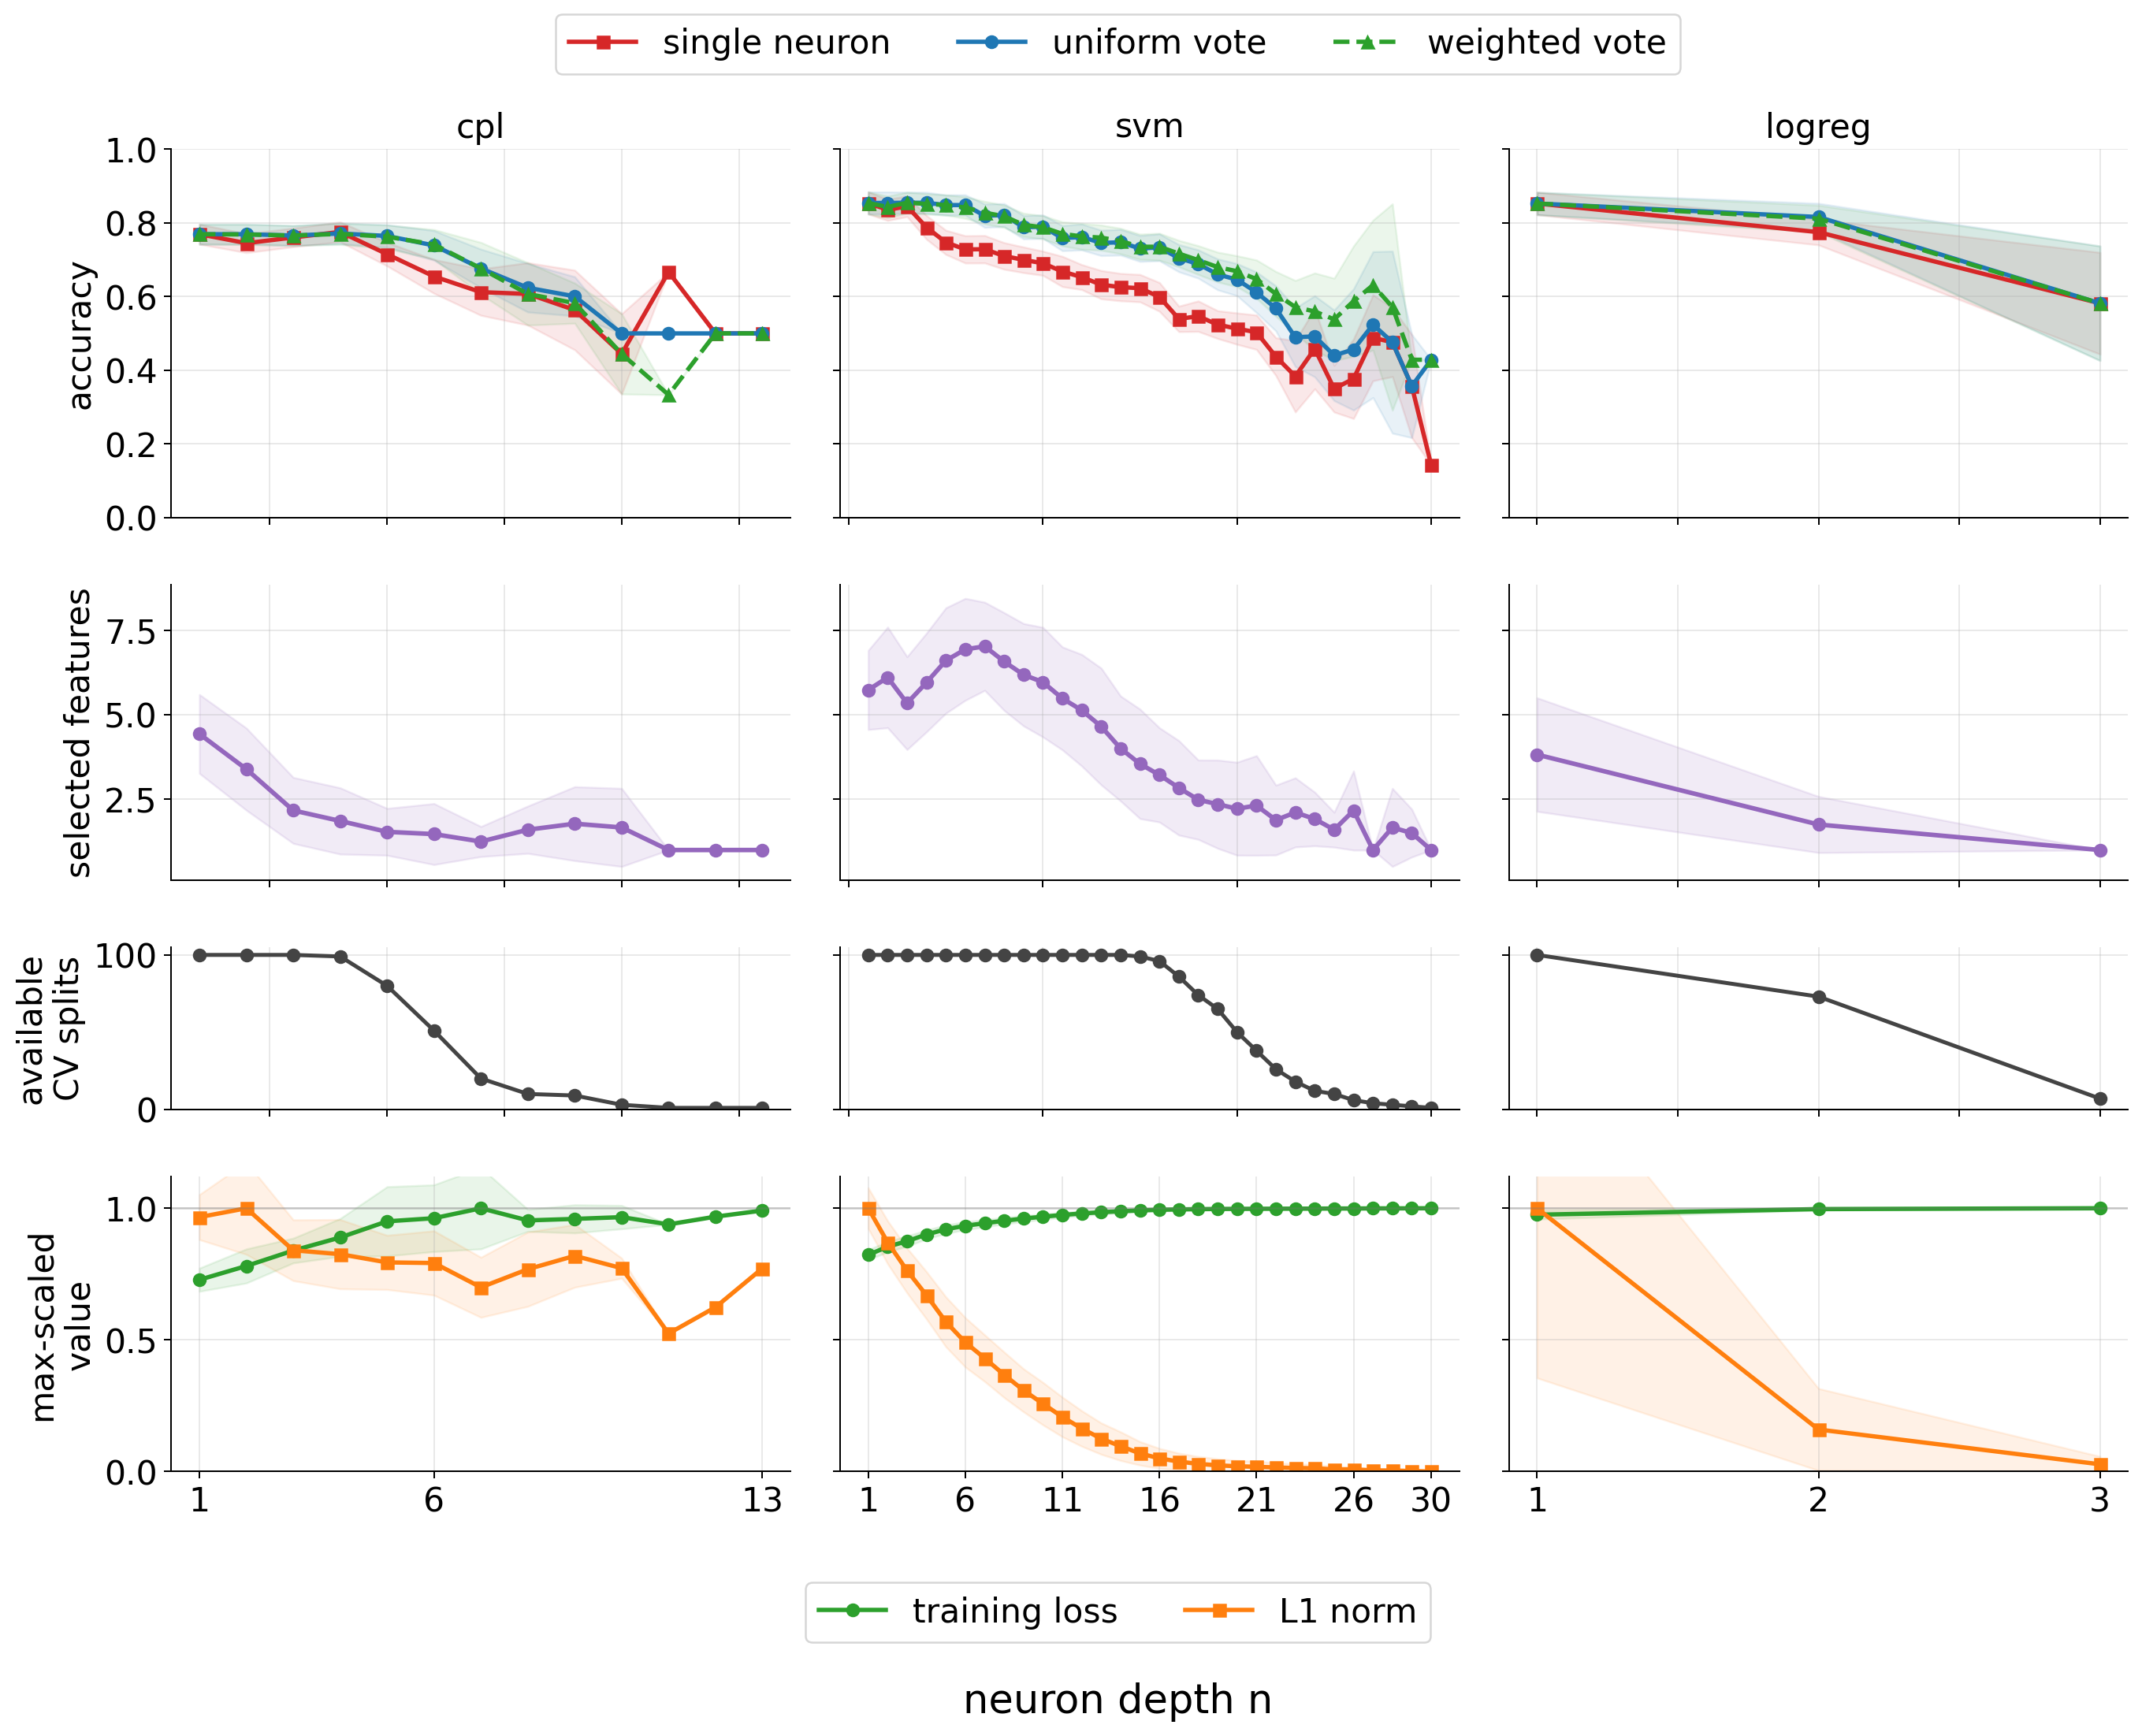
\includegraphics[width=\linewidth]{figures/paper_panels/colon_diagnostics_panel.png}
\caption{Low-feature diagnostic trajectories on the colon cancer benchmark. Columns show \texttt{cpl},
\texttt{svm}, and \texttt{logreg} with $C_{\mathrm{low}}$. Rows report predictive accuracy, the average number
of features selected by the $n$-th neuron, the number of CV splits in which that neuron depth was available,
and optimization diagnostics for the $n$-th neuron. Training loss and L1 norm are divided by their
within-model maximum values and should be interpreted as shape summaries rather than absolute-scale comparisons.}
\label{fig:colon_sparse_accuracy}
\end{figure}

\FloatBarrier

\subsection*{Synthetic predictive performance}
The synthetic benchmark first mirrors the colon cancer evaluation by comparing predictive trajectories across
learners and feature-count regimes. Its known ground truth is used separately below to analyze feature recovery.

\begin{table}[ht]
\centering
\small
\setlength{\tabcolsep}{3.5pt}
\begin{tabular}{llrr@{\hspace{1.8em}}rr@{\hspace{1.8em}}r}
\toprule
Model & Regime & \multicolumn{2}{c@{\hspace{1.8em}}}{$n=1$} & \multicolumn{2}{c@{\hspace{1.8em}}}{Best $n$} & Built \\
\cmidrule(lr){3-4}\cmidrule(lr){5-6}
 & & Features & Accuracy & $n$ & Accuracy & neurons \\
\midrule
\texttt{cpl} & $C_{\mathrm{low}}$ & 5.03 & 0.8180 & 3 & 0.8430 & 8 \\
\texttt{svm} & $C_{\mathrm{low}}$ & 6.42 & 0.8250 & 3 & 0.8500 & 8 \\
\texttt{logreg} & $C_{\mathrm{low}}$ & 3.44 & 0.6950 & 2 & 0.7424 & 3 \\
\midrule
\texttt{cpl} & $C_{\mathrm{high}}$ & 25.94 & 0.8160 & 3 & 0.8480 & 10 \\
\texttt{svm} & $C_{\mathrm{high}}$ & 25.32 & 0.8400 & 4 & 0.8490 & 13 \\
\texttt{logreg} & $C_{\mathrm{high}}$ & 27.58 & 0.8590 & 1 & 0.8590 & 7 \\
\bottomrule
\end{tabular}
\caption{Summary of the repeated-CV predictive results on the synthetic benchmark. The table follows the same
format as Table~\ref{tab:colon_summary}, reporting first-neuron width and accuracy, the best mean vote accuracy
and its depth, and the realized number of neurons.}
\label{tab:synthetic_performance}
\end{table}

In the low-feature regime, later neurons frequently improved predictive performance.
For \texttt{cpl} with $C_{\mathrm{low}}$, accuracy increased from 0.8180 at $n=1$ to 0.8430 at $n=3$, while
the first neuron selected 5.03 features on average.
For \texttt{svm} with $C_{\mathrm{low}}$, the best mean vote accuracy was 0.8500 at $n=3$, compared with 0.8250 at
$n=1$.
The first neuron selected 6.42 features on average.
For \texttt{logreg} with $C_{\mathrm{low}}$, the best result occurred at $n=2$, improving from 0.6950 at $n=1$ to
0.7424 at $n=2$.

In the high-feature regime, the first neuron often captured a larger fraction of the true signal, but additional
neurons contributed less useful information.
This was clearest for \texttt{logreg} with $C_{\mathrm{high}}$, where the first neuron already achieved the best mean
accuracy of 0.8590 and selected 27.58 features on average.
For \texttt{svm} with $C_{\mathrm{high}}$, the best mean accuracy was 0.8490 at $n=4$.
For \texttt{cpl} with $C_{\mathrm{high}}$, the best mean accuracy was 0.8480 at $n=3$.

Weighted voting again gave a more nuanced picture than a uniform improvement.
When only depths available in all 100 cross-validation splits were considered, the weighted vote reached the
same best accuracy as the unweighted vote for high-feature \texttt{logreg} (0.8590 at $n=1$), and a very similar
value for high-feature \texttt{svm} (0.8420 at $n=3$ versus an unweighted best of 0.8490 at $n=4$).
It did not improve the best accuracy of low-feature \texttt{cpl} or low-feature \texttt{svm}.
The clearest weighted-vote gain appeared for low-feature \texttt{logreg}, where the
weighted vote reached 0.7678 at $n=2$ compared with the unweighted value of 0.7424.

As for the colon cancer benchmark, the trajectory figures focus on the low-feature regime, where successive
neurons are most diagnostic of how predictive performance changes across depth. High-feature behavior is reported
in Table~\ref{tab:synthetic_performance} and in the text above.

\begin{figure}[!htbp]
\centering
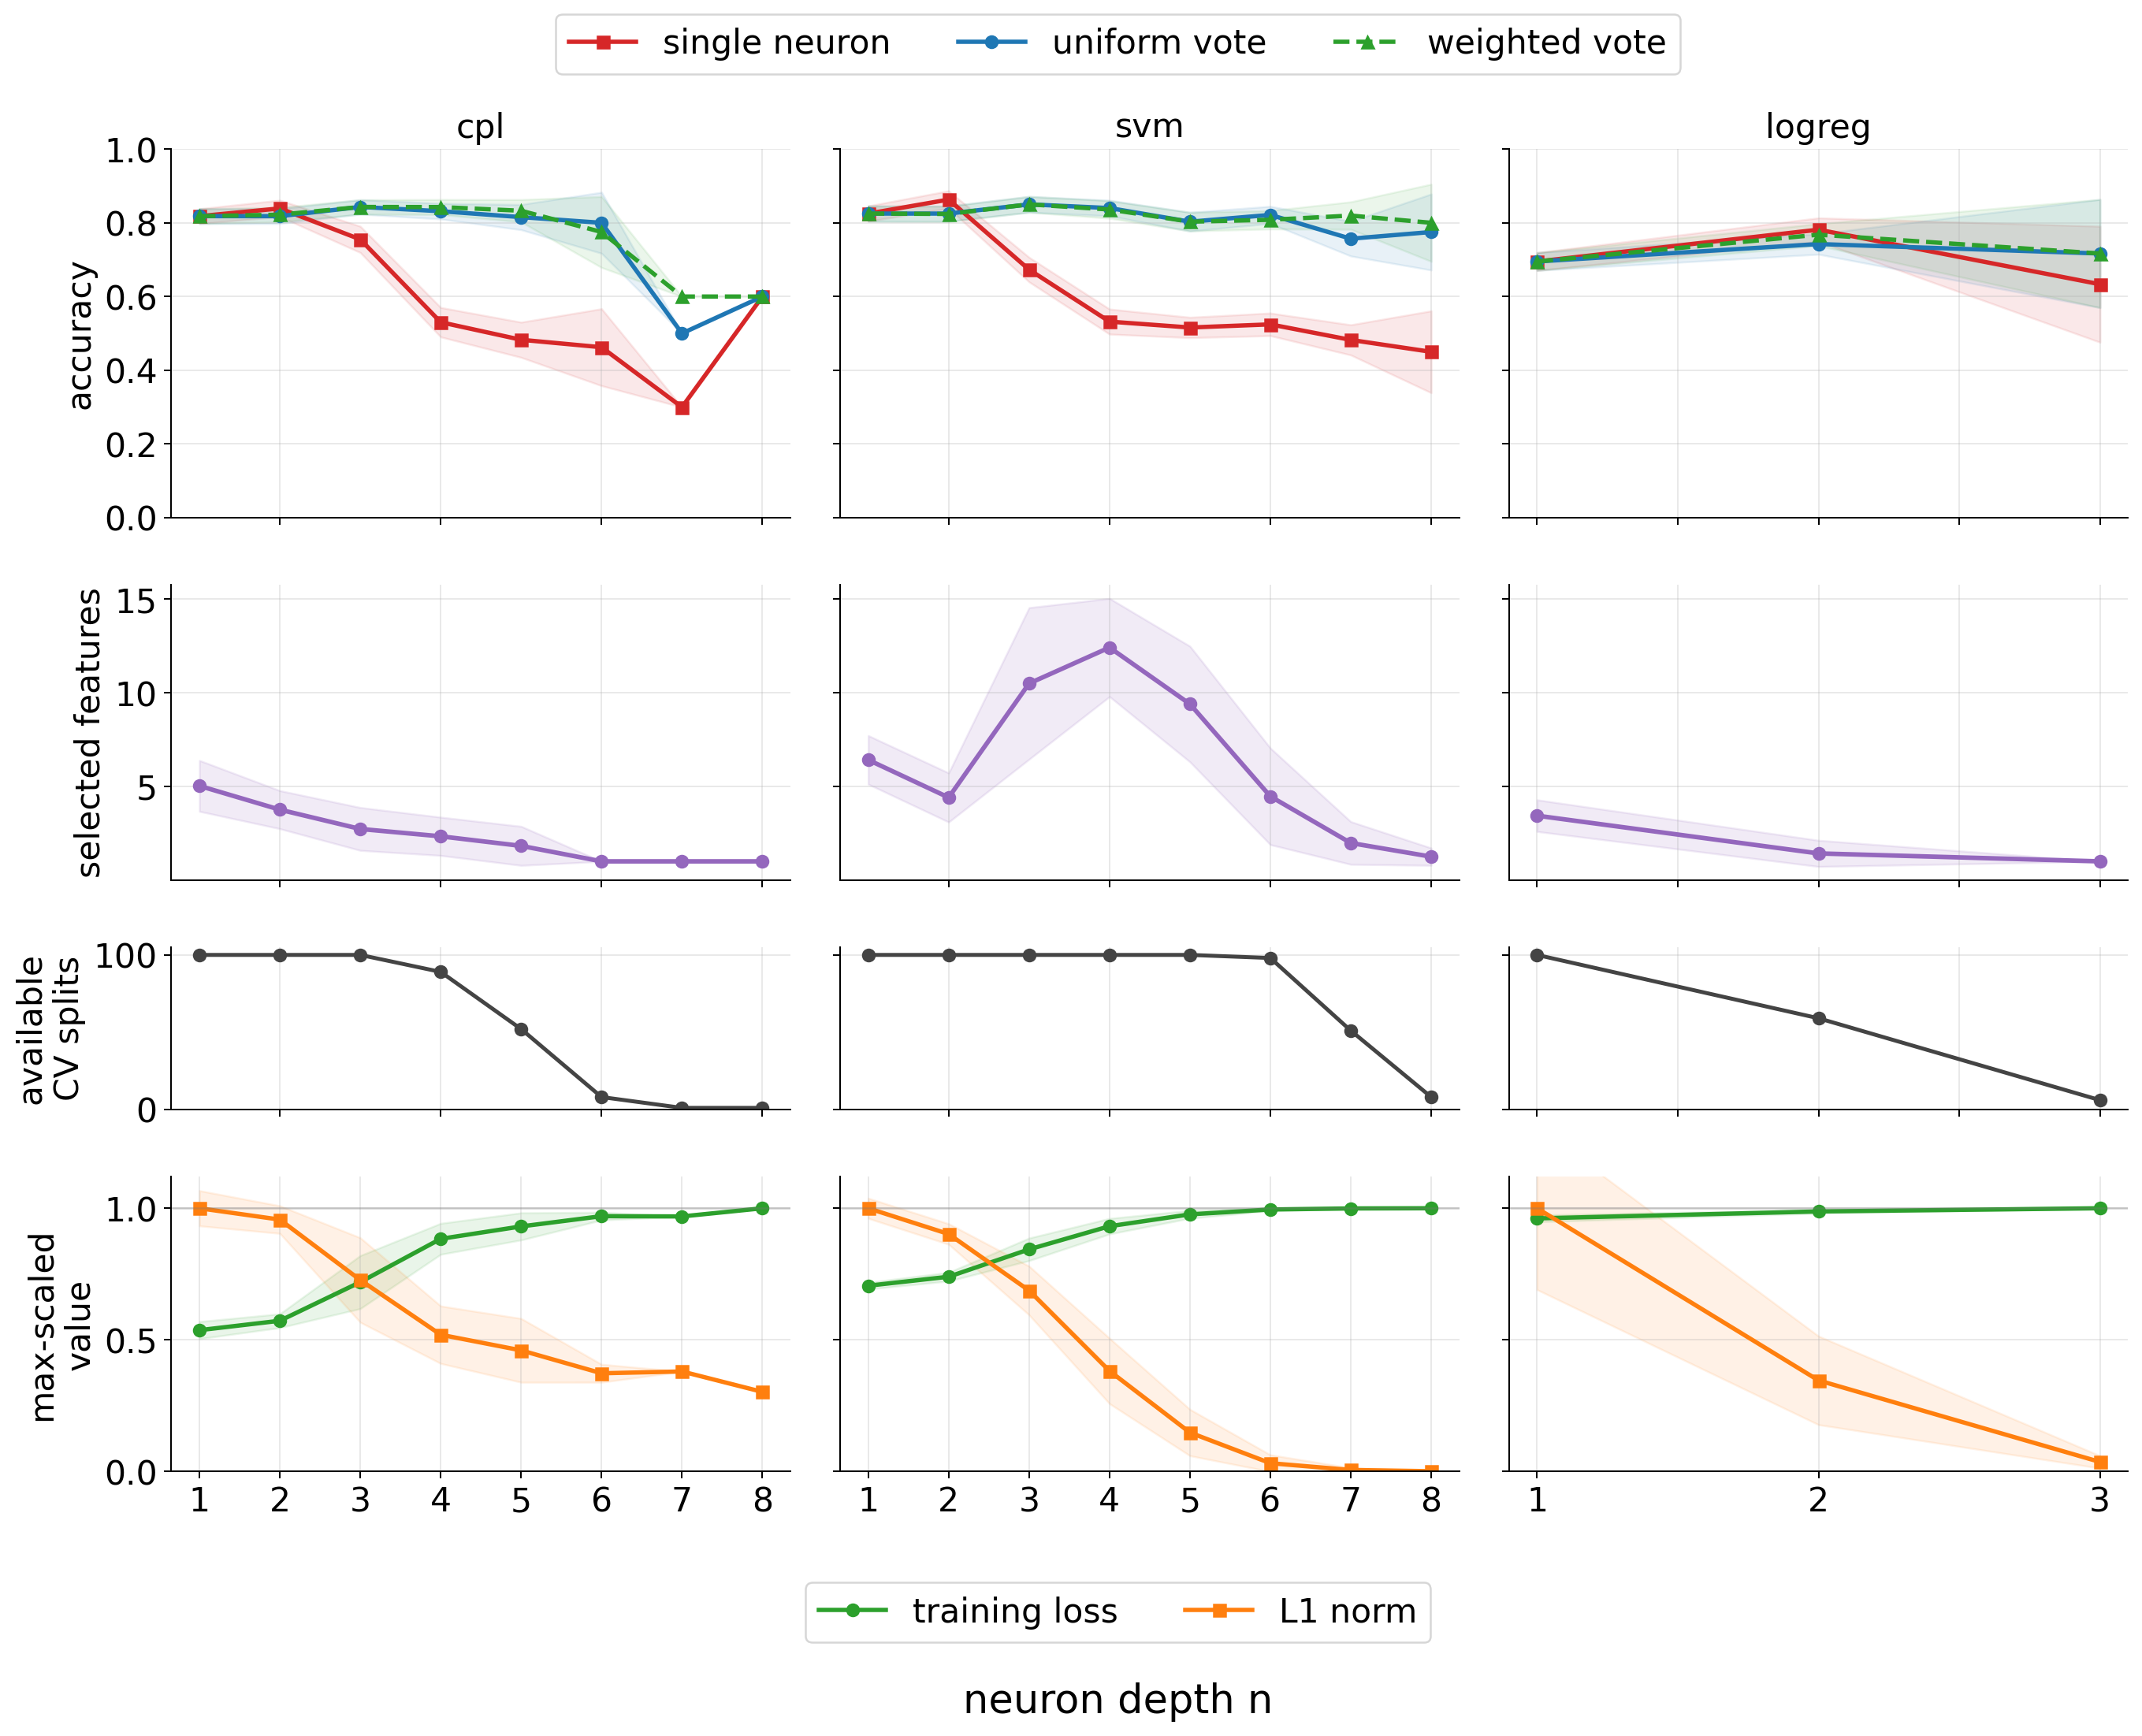
\includegraphics[width=\linewidth]{figures/paper_panels/synthetic_diagnostics_panel.png}
\caption{Low-feature diagnostic trajectories on the synthetic benchmark. Columns show \texttt{cpl},
\texttt{svm}, and \texttt{logreg} with $C_{\mathrm{low}}$. Rows report predictive accuracy, the average number
of features selected by the $n$-th neuron, the number of CV splits in which that neuron depth was available,
and optimization diagnostics for the $n$-th neuron. Training loss and L1 norm are divided by their
within-model maximum values and should be interpreted as shape summaries rather than absolute-scale comparisons.}
\label{fig:synthetic_sparse_accuracy}
\end{figure}

\FloatBarrier

\subsection*{Synthetic feature recovery}
The known informative-feature set in the synthetic benchmark makes it possible to ask whether predictive gains
come from recovering true signal or from selecting broader sets of noisy features.

\begin{table}[ht]
\centering
\small
\setlength{\tabcolsep}{4pt}
\begin{tabular}{llrr@{\hspace{1.8em}}rrr}
\toprule
Model & Regime & \multicolumn{2}{c@{\hspace{1.8em}}}{$n=1$} & \multicolumn{3}{c}{Cumulative at Best $n$} \\
\cmidrule(lr){3-4}\cmidrule(lr){5-7}
 & & Precision & Recall & $n$ & Precision & Recall \\
\midrule
\texttt{cpl} & $C_{\mathrm{low}}$ & 0.6497 & 0.2617 & 3 & 0.6923 & 0.6475 \\
\texttt{svm} & $C_{\mathrm{low}}$ & 0.6425 & 0.3367 & 3 & 0.4114 & 0.6908 \\
\texttt{logreg} & $C_{\mathrm{low}}$ & 1.0000 & 0.2867 & 2 & 1.0000 & 0.3686 \\
\midrule
\texttt{cpl} & $C_{\mathrm{high}}$ & 0.1880 & 0.4033 & 3 & 0.1413 & 0.7767 \\
\texttt{svm} & $C_{\mathrm{high}}$ & 0.2040 & 0.4267 & 4 & 0.0788 & 0.9167 \\
\texttt{logreg} & $C_{\mathrm{high}}$ & 0.3167 & 0.7217 & 1 & 0.3167 & 0.7217 \\
\bottomrule
\end{tabular}
\caption{Informative-feature recovery on the synthetic benchmark. The $n=1$ columns report precision and recall
for the first neuron alone. The cumulative columns are computed over all features selected up to the
best-accuracy depth reported in Table~\ref{tab:synthetic_performance}.}
\label{tab:synthetic_recovery_summary}
\end{table}

These recovery summaries separate two modes of behavior.
Some models, especially high-feature \texttt{logreg}, concentrate much of the ground-truth signal in the first
neuron. Other configurations, including low-feature \texttt{cpl} and \texttt{svm}, recover informative structure
more gradually across successive neurons before later neurons become dominated by noise features.

\begin{figure}[!htbp]
\centering
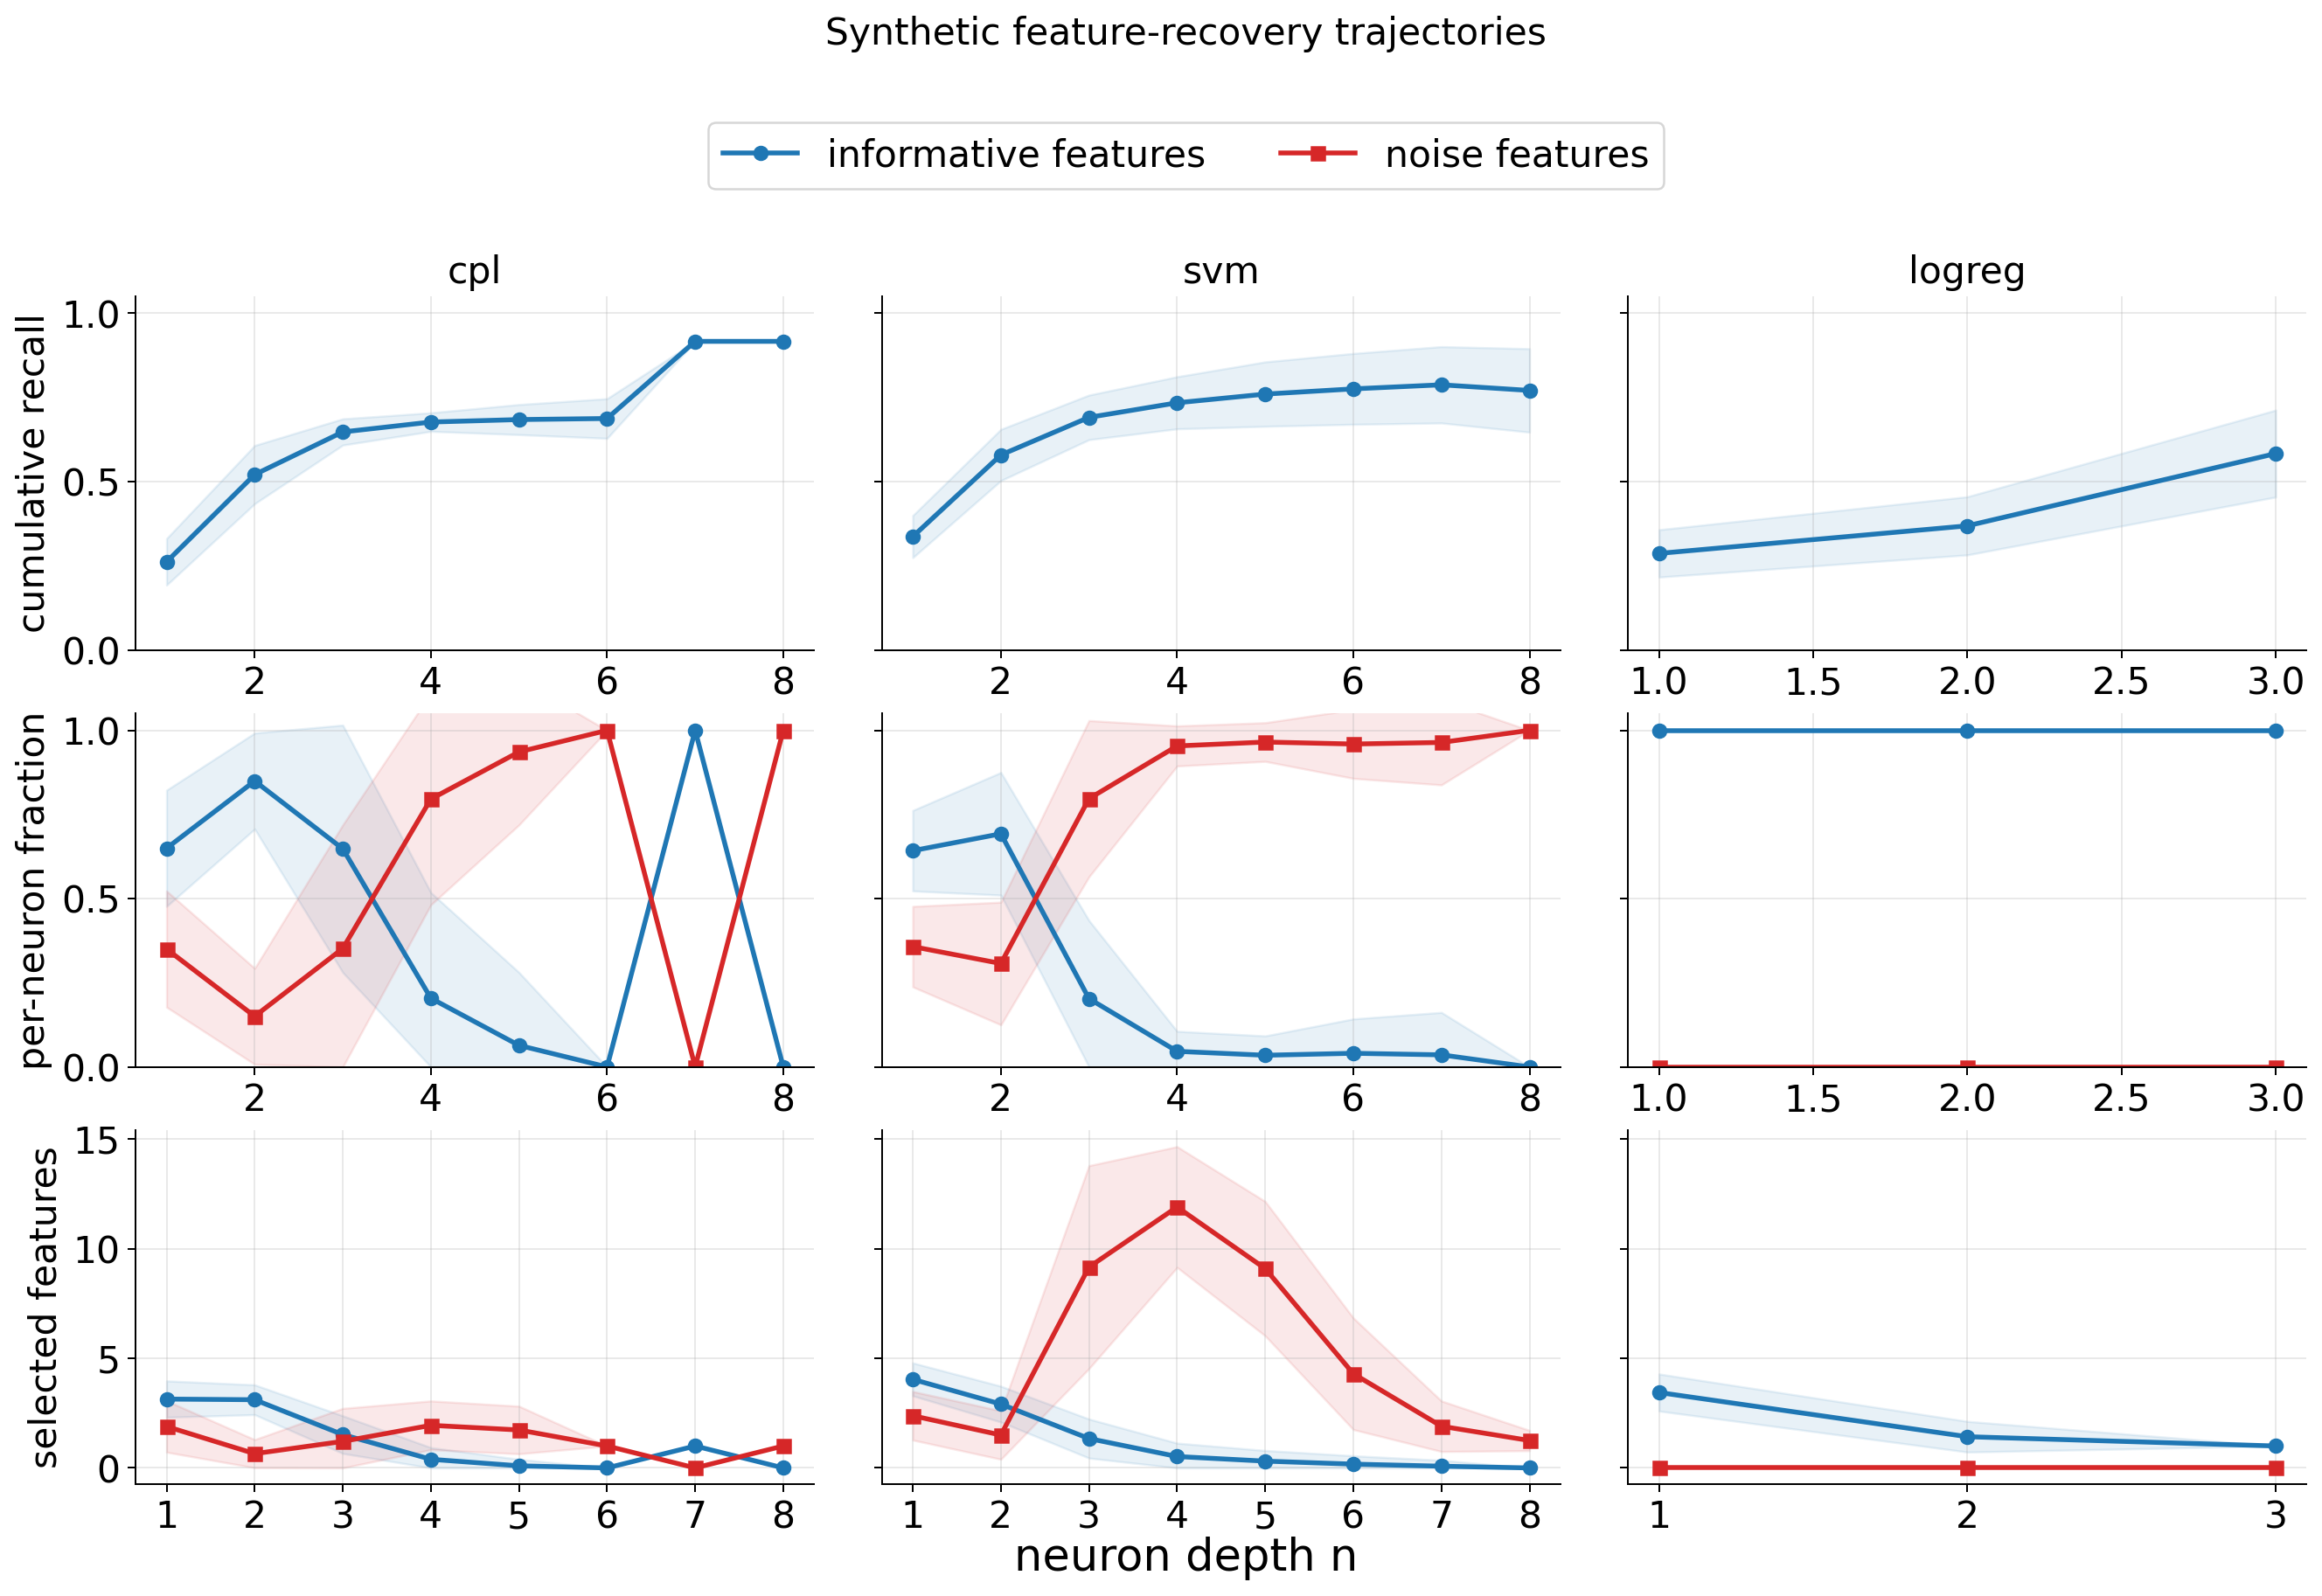
\includegraphics[width=\linewidth]{figures/paper_panels/synthetic_recovery_panel.png}
\caption{Feature-recovery trajectories for the low-feature synthetic benchmark. Columns show \texttt{cpl},
\texttt{svm}, and \texttt{logreg} with $C_{\mathrm{low}}$; rows report cumulative informative-feature recall,
per-neuron informative and noise fractions, and the numbers of informative and noise features selected by the
$n$-th neuron. Blue trajectories describe informative features and red trajectories describe noise features.}
\label{fig:synthetic_sparse_recovery}
\end{figure}

\FloatBarrier

\subsection*{Built depth as a model property}
The nominal maximum depth was 31 neurons, but the realized depth depended strongly on the learner and
regularization.
On the colon cancer benchmark, the realized depth ranged from 3 neurons for low-feature \texttt{logreg} to 31 neurons
for high-feature \texttt{cpl} and high-feature \texttt{svm}.
On the synthetic benchmark, realized depth was markedly smaller, ranging from 3 neurons for low-feature
\texttt{logreg} to 13 neurons for high-feature \texttt{svm}.
This supports the view that neuron depth is not only a reporting axis but also an empirical signature of how
aggressively each base learner exhausts the remaining feature space.

\section*{Discussion}

The final experiments support a narrower and more defensible interpretation of complex layers than a simple
claim that voting should monotonically improve classification.
Across both datasets, the most useful information was typically concentrated in the first few neurons, but
the exact pattern depended on the base learner and on the feature-count regime induced by regularization.

The real-data benchmark showed that later neurons can be useful, but only modestly and not uniformly.
On \texttt{colon\_cancer}, \texttt{cpl} and \texttt{svm} reached their best mean accuracies after several neurons,
whereas \texttt{logreg} was already best at the first neuron in both feature-count regimes.
This suggests that sequential feature removal can expose complementary predictive structure for some learners,
but it should not be interpreted as a general guarantee that deeper voting improves accuracy.
The high-feature regime also showed that broader first neurons do not necessarily exhaust the constructible
sequence: although they selected more features initially, weaker effective regularization allowed later nonzero
neurons to be fitted in many splits.

The synthetic benchmark clarifies why these regimes differ.
When the first neuron is broad, as in high-feature \texttt{logreg}, it can recover a large fraction of the true
signal at once, but later neurons contribute little additional information.
When the first neuron is narrower, as in low-feature \texttt{cpl} or \texttt{svm}, recovery of informative
features is more gradual, and meaningful gains may emerge only after several neurons.
This makes neuron depth a useful analytical dimension for studying how a learner decomposes signal, rather
than merely an aggregation mechanism.
The low-feature \texttt{logreg} result also illustrates why later-depth summaries must be interpreted together
with coverage.
Its apparent improvement at $n=2$ reflects the subset of cross-validation splits in which a second neuron could
be fitted; within those splits, the unweighted two-neuron vote is identical to the first-neuron prediction under
the tie-breaking rule.
Thus, available-split counts are part of the result rather than only a plotting diagnostic.

Across both benchmarks, training-based weighted voting changed the conclusions little.
The weighted and uniform vote trajectories were usually close, indicating that the main effect came from the
successive sparse fits and the changing feature pool, not from the particular vote-weighting scheme.

The comparison also exposes a recurring trade-off between signal recovery and feature purity.
Broader neurons often recovered a larger share of informative variables, but they also selected many noisy
features.
Narrower neurons were cleaner, but they could require several layers before accumulating comparable signal.
This trade-off is central to the interpretation of later neurons and should be reported explicitly rather than
collapsed into a single accuracy score, in line with broader feature-selection literature
\cite{saeys2007review,nogueira2018stability}.

An additional practical observation is that realized depth itself is informative.
Some colon cancer configurations reached the nominal limit of 31 neurons, whereas the synthetic configurations
terminated after 3--13 neurons.
This suggests that the number of constructible neurons is not a trivial implementation detail; it reflects how
fast the learner exhausts separable structure under the imposed regularization.

Key limitations remain.
\begin{itemize}[noitemsep]
\item \texttt{colon\_cancer} is a small and classical microarray dataset, so its statistical variability is
high.
\item The synthetic benchmark is informative because it provides ground truth, but its conclusions remain
conditional on the chosen latent-source data-generation process.
\item Regularization values were calibrated to obtain comparable first-neuron widths, not to equalize the
effective penalty across models; direct numerical comparison of $C$ between learners is therefore not
meaningful.
\item The present study does not perform nested model selection, so the reported settings should be interpreted
as controlled analysis regimes rather than globally optimal hyperparameters.
\end{itemize}

Future work should extend this analysis to additional high-dimensional biological datasets, investigate the
stability of neuron-wise feature recovery across repeated resampling \cite{lukaszuk2024importance}, and study whether alternative stopping
rules can identify the depth at which complementary signal is exhausted and later neurons become primarily
noise-driven.

\section*{Conclusions}

We provide a reproducible comparative protocol for layered sparse linear classifiers on a real microarray
benchmark and a synthetic benchmark with known signal structure. Under repeated cross-validation, the three
analyzed methods (\texttt{cpl}, \texttt{svm}, \texttt{logreg}) can now be compared not only in terms of
predictive behavior across neuron depths and training-quality weighted voting, but also in terms of how quickly
they recover truly informative features and how rapidly later neurons become noise-dominated. The presented
protocol supports transparent, repeatable comparisons in which neuron depth is treated as an object of
analysis, not merely as a route to a final voted classifier.

The implemented model type is deliberately sparse and linear. This choice is justified by the small-sample,
high-dimensional setting: sparse formal neurons keep the selected feature sets inspectable, while the
complex-layer construction makes it possible to study whether successive sparse neurons expose complementary
signal after earlier selected features are removed. The comparison with sparse \texttt{svm} and
\texttt{logreg} baselines shows that this behavior depends on the loss function and the induced feature-count
regime, not only on the voting mechanism.

The main limitations are the small size of the real microarray benchmark, the controlled but necessarily
simplified synthetic data-generation process, and the use of calibrated analysis regimes rather than nested
hyperparameter selection. Future work should repeat the protocol on additional high-dimensional biological
datasets, study the stability of neuron-wise selected features, and develop stopping rules for identifying
when later neurons have become primarily noise-driven.


\section*{Acknowledgements}
This article is the outcome of collaboration developed during Jerzy Krawczuk's research internship at the
Institute of Biocybernetics and Biomedical Engineering, Polish Academy of Sciences, under the supervision of
Professor Leon Bobrowski.

\section*{Additional Information and Declarations}
\subsection*{Funding}
This work was supported by the grant WZ/WI-IIT/4/2026 from Bialystok University of Technology.

\subsection*{Competing Interests}
The authors declare there are no competing interests.

\subsection*{Author Contributions}
Jerzy Krawczuk conceived the study, implemented the experimental protocol, performed the experiments,
analyzed the results, and drafted the manuscript.

\noindent
Leon Bobrowski developed the theoretical framework, supervised the study, interpreted the results,
and revised the manuscript critically.

\noindent
Both authors approved the final draft.

\subsection*{Data Availability}
The materials needed to reproduce the analyses, including source code, input datasets, result tables, and
figure-generation materials, are available in the project repository archived at [DOI to be added before
submission].
The colon cancer benchmark used in this study corresponds to the Alon et al. (1999) microarray dataset
distributed by the Bioconductor \texttt{colonCA} experiment data package (DOI:
\texttt{10.18129/B9.bioc.colonCA}; LGPL). It is included in the archived repository as the processed
\texttt{data/colon\_cancer.csv} file used for the experiments; this data file follows the upstream
\texttt{colonCA} LGPL package license and is not covered by the repository MIT code license.

\subsection*{Supplemental Information}
Supplemental material for submission should include the archived analysis materials, machine-readable result
tables, and figure-generation materials.

\subsection*{Additional Declarations}
Jerzy Krawczuk used generative AI assistance during manuscript preparation. The AI system was used for
language editing, restructuring of selected manuscript sections, coding assistance related to the experimental
protocol, and preparation of draft figure and table arrangements. All scientific decisions, experimental
design choices, result interpretation, and final manuscript revisions were made and verified by the authors.

\bibliography{references}

\end{document}
